\newcommand{\prompttag}[1]{\textcolor{blue}{\texttt{<|#1|>}}}

\section{Model Training Details}\label{ch2:sec:training}

The implemented training lineage contains four paper-level models. The pretrained
base model is denoted \textit{Model chk-0}. Supervised fine-tuning (SFT) on
point-in-time evidence-to-analysis pairs produces \textit{Model chk-1}, which
serves as the common parent of two independent downstream branches.
\textit{Model chk-2} (repository artifact \texttt{chk3}, checkpoint 318) is
obtained by supervised fine-tuning \textit{Model chk-1} on the
analysis-to-FOMC-Minutes rewriting task. \textit{Model chk-3} (repository
artifact \texttt{chk4}) is obtained through a separate policy-decision branch:
decision-specific SFT at checkpoint 38 initializes GRPO, whose completed run
ends at step 468. Checkpoint 450 is retained only as the best-observed
exploratory post-GRPO evaluation candidate. The authoritative selection record
has \texttt{selected\_checkpoint\_step=null}, and the subsequent test verdict is
\texttt{quality\_not\_demonstrated}; checkpoint 450 is therefore not a selected,
final, or promoted model. Checkpoint 38 is the intermediate pre-GRPO state of
\textit{Model chk-3}, not a separate paper-level model, and
\textit{Model chk-3} does not consume outputs generated by \textit{Model
chk-2}. Figure~\ref{fig:ch2:training_stage1} summarizes this lineage.

\begin{figure}[htbp]
    \centering
    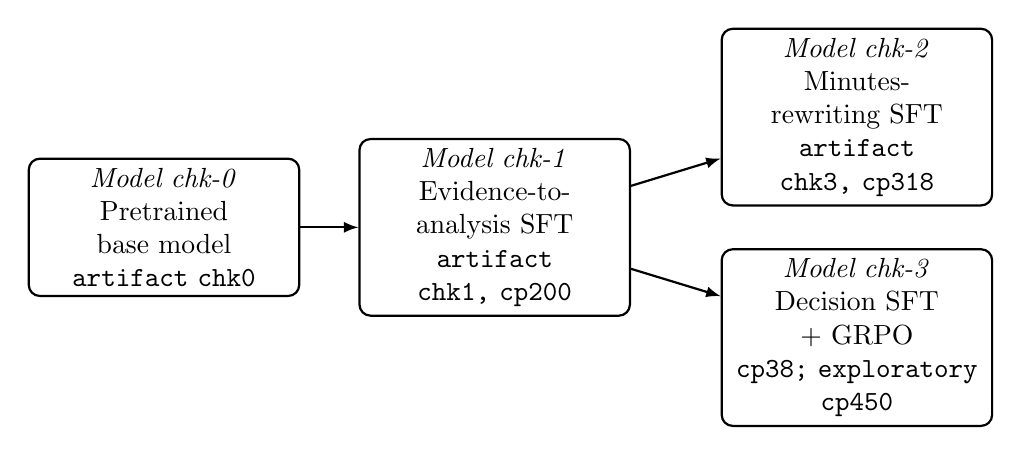
\begin{tikzpicture}[
        >=latex,
        model/.style={draw, rounded corners, align=center, text width=3.2cm,
            minimum height=1.45cm},
        every path/.style={->, thick}
    ]
        \node[model] (chk0) at (0,0)
            {\textit{Model chk-0}\\Pretrained base model\\\texttt{artifact chk0}};
        \node[model] (chk1) at (4.2,0)
            {\textit{Model chk-1}\\Evidence-to-analysis SFT\\\texttt{artifact chk1, cp200}};
        \node[model] (chk2) at (8.8,1.4)
            {\textit{Model chk-2}\\Minutes-rewriting SFT\\\texttt{artifact chk3, cp318}};
        \node[model] (chk3) at (8.8,-1.4)
            {\textit{Model chk-3}\\Decision SFT + GRPO\\\texttt{cp38; exploratory cp450}};
        \draw (chk0) -- (chk1);
        \draw (chk1) -- (chk2);
        \draw (chk1) -- (chk3);
    \end{tikzpicture}
    \caption{Paper-level training lineage and repository-artifact mapping.}
    \label{fig:ch2:training_stage1}
\end{figure}


%SFT
\paragraph*{Supervised fine-tuning.}
SFT adapts the model to the macro-financial tasks by learning from paired
prompts and reference completions. Each training example contains a system
instruction, a user prompt, and a target assistant response. The model is
optimized under teacher forcing, while parameter-efficient adapters reduce
the number of trainable parameters. Figure~\ref{fig:ch2:ft_detail} summarizes
this workflow.


\begin{figure}
    \begin{center}
        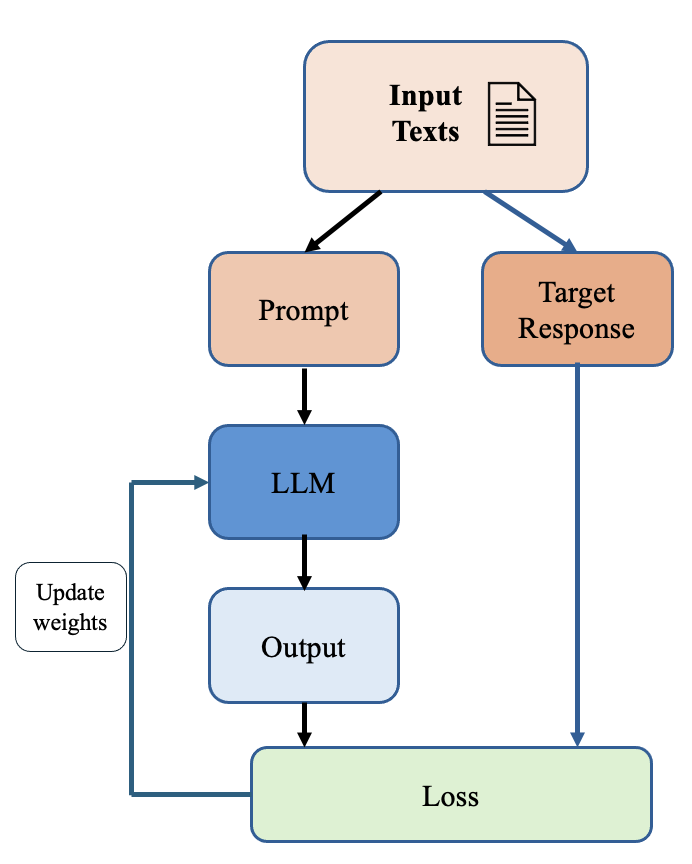
\includegraphics[width=0.3\textwidth]{Chapter2/Chapter2Figs/ft_detail.png}
      \end{center}
      \caption{Supervised fine-tuning workflow.}
      \label{fig:ch2:ft_detail}
\end{figure}



During SFT, let $x=(x_1,\ldots,x_M)$ denote the serialized prompt and
$y=(y_1,\ldots,y_N)$ the target assistant completion. At each target
position, the model predicts a distribution over the vocabulary conditional
on the prompt and preceding target tokens. The mean token-level negative
log-likelihood is
\begin{equation}
    \mathcal{L}_{\mathrm{SFT}}(\theta)
    =
    -\frac{1}{W}
    \sum_{t=1}^{N}
    w_t
    \log \pi_\theta\!\left(y_t\mid x,y_{<t}\right),
    \qquad
    W=\sum_{t=1}^{N}w_t,
\end{equation}
where $w_t\in\{0,1\}$ masks padding and any positions excluded from the
supervised objective. If every completion token is trained, $w_t=1$ and
$W=N$. Thus, SFT minimizes the negative log-probability assigned to the
reference completion; it does not compare a separately decoded response with
the target text.


%RL
\paragraph*{Reinforcement learning.}
Unlike SFT, policy optimization does not require a token-level reference
completion. In the decision task, however, the reference action remains
available to the deterministic reward function: the policy sees the prompt,
whereas the target direction and magnitude are used only to score sampled
completions.

Proximal Policy Optimization (PPO; \cite{schulman2017proximal}) stabilizes
policy-gradient updates by clipping the importance-sampling ratio. Let
$s_t=(q,o_{<t})$ be the token-generation state and define
\begin{equation*}
    \rho_t(\theta)
    =
    \frac{\pi_\theta(o_t\mid s_t)}
         {\pi_{\theta_{\mathrm{old}}}(o_t\mid s_t)}.
\end{equation*}
The clipped policy objective is
\begin{equation}
    \mathcal{J}_{\mathrm{PPO}}(\theta)
    =
    \mathbb{E}_t\!\left[
        \min\!\left(
            \rho_t(\theta)\widehat{A}_t,
            \operatorname{clip}
            \bigl(\rho_t(\theta),1-\epsilon,1+\epsilon\bigr)
            \widehat{A}_t
        \right)
    \right].
\end{equation}
Here, $\widehat{A}_t$ is an advantage estimate rather than the reward itself;
clipping constrains the policy ratio rather than rescaling the reward.




GRPO (\cite{shao2024deepseekmath}) removes the learned value function. For
each prompt $q$, the behavior policy samples a group
$\{o_i\}_{i=1}^{G}$, and the task reward assigns one terminal score
$R_i=R(q,y,o_i)$ to each completion. The group-relative advantage is
\begin{equation}
    \widehat{A}_i
    =
    \begin{cases}
    \displaystyle\frac{R_i-\overline{R}}{s_R+\eta}, & s_R>0,\\[7pt]
    0, & s_R=0,
    \end{cases}
    \qquad
    \overline{R}=\frac{1}{G}\sum_{j=1}^{G}R_j,
\end{equation}
where $s_R$ is the within-group reward standard deviation and $\eta>0$ is a
numerical stabilizer. The same completion-level advantage is applied to every
generated token in $o_i$. A group whose completions all receive the same
reward therefore supplies no group-relative learning signal.




For token $t$ of completion $i$, define
\begin{equation*}
    \rho_{i,t}(\theta)
    =
    \frac{\pi_\theta(o_{i,t}\mid q,o_{i,<t})}
         {\pi_{\theta_{\mathrm{old}}}(o_{i,t}\mid q,o_{i,<t})}.
\end{equation*}
A sampled per-token estimator for the KL regularizer is
\begin{equation*}
    \widehat{D}_{\mathrm{KL},i,t}
    =
    \frac{\pi_{\mathrm{ref}}(o_{i,t}\mid q,o_{i,<t})}
         {\pi_\theta(o_{i,t}\mid q,o_{i,<t})}
    -\log
    \frac{\pi_{\mathrm{ref}}(o_{i,t}\mid q,o_{i,<t})}
         {\pi_\theta(o_{i,t}\mid q,o_{i,<t})}
    -1.
\end{equation*}
Using
\begin{equation*}
    \ell_{i,t}(\theta)
    =
    \min\!\left(
        \rho_{i,t}(\theta)\widehat{A}_i,
        \operatorname{clip}
        \bigl(\rho_{i,t}(\theta),1-\epsilon,1+\epsilon\bigr)
        \widehat{A}_i
    \right)
    -\beta\widehat{D}_{\mathrm{KL},i,t},
\end{equation*}
the original sequence-normalized GRPO objective can be written as
\begin{equation}
    \mathcal{J}_{\mathrm{GRPO}}(\theta)
    =
    \mathbb{E}\!\left[
        \frac{1}{G}\sum_{i=1}^{G}
        \frac{1}{|o_i|}\sum_{t=1}^{|o_i|}
        \ell_{i,t}(\theta)
    \right].
\end{equation}

The completed decision run instead sets \texttt{loss\_type=dapo}. In this
trainer setting, DAPO denotes token-level loss aggregation: the losses are
normalized by the number of active completion tokens in the accumulated
training batch rather than separately by each completion length. If
$\mathcal{C}$ is the set of unmasked completions in that batch, the realized
aggregation is
\begin{equation}
    \mathcal{J}_{\mathrm{DAPO}}(\theta)
    =
    \mathbb{E}\!\left[
        \frac{\displaystyle
            \sum_{i\in\mathcal{C}}\sum_{t=1}^{|o_i|}\ell_{i,t}(\theta)}
             {\displaystyle
            \sum_{i\in\mathcal{C}}|o_i|}
    \right].
\end{equation}
This setting is related to the token-level aggregation proposed in DAPO
(\cite{yu2025dapo}), but it does not imply that the run adopted the complete
DAPO recipe. The realized configuration retained symmetric clipping and a KL
penalty; its numerical settings are reported with the decision-training
configuration below.





\subsection*{Analytical and Downstream Training}

\subsubsection*{Supervised Fine-tuning for the Analytical Model}

\paragraph*{Model chk-1.}
The first SFT stage adapts \textit{Model chk-0} to point-in-time
macro-financial analysis. Each supervised example is a pair
$(q_i,o_i^{\mathrm{SFT}})$, where $q_i$ is the model-visible prompt and
$o_i^{\mathrm{SFT}}=(c_i,a_i)$ is the reference assistant completion. Here,
$c_i$ denotes the reasoning prefix and $a_i$ the concise final analysis. This
distinction separates the model input from the supervision target. Training
for a small number of epochs limits, but does not eliminate, the risk that the
model memorizes task-specific wording.



Moreover, each LLM requires a model-specific message format, because tokenizers encode role boundaries differently. Explicit role labels are used specifically to distinguish the sections: the ``\texttt{System Prompt}'', ``\texttt{User Prompt}'', and ``\texttt{Assistant Response}''. Table. \ref{tab:ch2:input_template_for_llama3} presents the labels used by LLAMA3, where ``\prompttag{start\_header\_id}'' and ``\prompttag{end\_header\_id}'' wrap around the role labels indicating the message type. The label ``\prompttag{begin\_of\_text}'' signals the start of the conversation, while ``\prompttag{end\_id}'' denotes its end.



\begin{table}[h]
    \centering
    \footnotesize
    \begin{tabular}{p{0.98\textwidth}}
    \toprule
    \textbf{Special Labels for LLaMA 3:} \\
    \midrule
    \prompttag{begin\_of\_text} \\
    \prompttag{start\_header\_id} \textcolor{red}{system}\prompttag{end\_header\_id} \\
    \texttt{... System Prompts ...} \\
    \prompttag{start\_header\_id} \textcolor{red}{user}\prompttag{end\_header\_id} \\
    \texttt{... User Prompts ...} \\
    \prompttag{start\_header\_id} \textcolor{red}{assistant}\prompttag{end\_header\_id} \\
    \texttt{... Assistant Response ...} \\
    \prompttag{end\_id} \\
    \bottomrule
    \end{tabular}
    \caption{Input Template for LLAMA3}
    \label{tab:ch2:input_template_for_llama3}
\end{table}



\paragraph*{Reasoning boundary and final answer.}
The supervised completions follow the model's native reasoning-boundary
convention. A nonempty reasoning prefix $c_i$ is followed by exactly one
literal \texttt{</think>} marker and a nonempty final
answer $a_i$. Writing the boundary token as $b_{\mathrm{think}}$, the
serialized completion is
\begin{equation*}
    o_i=c_i\;\Vert\;b_{\mathrm{think}}\;\Vert\;a_i,
\end{equation*}
where $\Vert$ denotes string concatenation. The serialized targets do not add
an opening \texttt{<think>} tag or \texttt{<answer>} tags. The semantic form
of $a_i$ is task-specific: prose for \textit{Models chk-1 and chk-2},
and a decision JSON object for \textit{Model chk-3}. The system prompt in
Table~\ref{tab:ch2:system_prompt} states this shared boundary contract.


\begin{table}[htbp]
    \centering
    \footnotesize
    \begin{tabular}{@{}p{\textwidth}@{}}
    \toprule
    \textbf{System Prompt:} \\
    \midrule
      Use the supplied evidence and task instructions only. Produce a substantive reasoning prefix, close it with exactly one \texttt{</think>} boundary, and then provide the task-specific final answer. Do not add an opening \texttt{<think>} tag or \texttt{<answer>} tags. \\
    \bottomrule
    \end{tabular}
    \caption{Shared native reasoning-boundary instruction.}
    \label{tab:ch2:system_prompt}
\end{table}


\paragraph*{Example SFT instance for \textit{Model chk-1}.}
Table~\ref{tab:chk1-sft-example} shows one evidence-to-analysis training
example using the shared boundary contract.

\begin{table}[!tbp]
\centering
\footnotesize
\caption{Example of a supervised fine-tuning instance for \textit{Model chk-1}.}
\label{tab:chk1-sft-example}
\renewcommand{\arraystretch}{1.25}
\setlength{\tabcolsep}{8pt}

\begin{tabularx}{\textwidth}{@{}
    >{\raggedright\arraybackslash}X
@{}}
\toprule

\textbf{System Prompt} \\[2pt]
Analyze only the supplied point-in-time FOMC evidence.
Do not infer facts from later releases or from the target meeting's Minutes.
Use the model's native reasoning boundary, then provide a concise,
evidence-grounded final analysis.
\\

\midrule

\textbf{User Prompt} \\[2pt]
Analyze the supplied point-in-time evidence for the atomic topic below.
Use the supplied FOMC section style, remain neutral, and do not add external
events, people, policy actions, causes, or post-cutoff facts.
Every number and directional statement must be grounded in the fact card.
Think first, then provide a concise final analysis.

\par\medskip
\textbf{Atomic topic:} Unemployment Rate.

\par\smallskip
\textbf{Fact card:}
The unemployment rate was 8.5\% in March 2009, increased to 8.9\% in April
2009, and reached 9.4\% in May 2009. The May observation was the latest
available value. The source series was \texttt{UNRATE}, measured in percent,
with availability governed by the sealed ALFRED day-one upper-bound rule.

\par\smallskip
\textbf{Style guidance:}
Use neutral third-person prose. Begin with an aggregate evidence-based
observation, order the discussion from recent movement to broader comparison,
use restrained contrast, and qualify uncertainty. Do not introduce named
individuals, meeting-specific events, or policy outcomes.
\\

\midrule

\textbf{Target Response} \\[2pt]
The available observations indicate that the unemployment rate continued to
rise over the period covered by the data. It increased in every successive
month, and the latest observation was also the highest. This pattern points to
persistent labor-market deterioration rather than stabilization. However, the
evidence covers only three monthly observations, so the conclusion should
remain limited to the observed period.

\par\smallskip
\texttt{</think>}

\par\smallskip
The unemployment rate continued to rise, moving from 8.5 percent in March to
8.9 percent in April and reaching 9.4 percent in May, suggesting persistent
labor-market weakness.
\\

\bottomrule
\end{tabularx}
\end{table}







\subsubsection*{Further Training for Downstream Tasks}

We adapt \textit{Model chk-1} separately for two downstream tasks. SFT on
analysis-to-FOMC-Minutes-style paragraph pairs produces \textit{Model chk-2}.
A separate branch uses decision SFT followed by GRPO to produce
\textit{Model chk-3}, which predicts the direction and magnitude of a federal
funds rate action. The two branches share \textit{Model chk-1} as their parent,
but neither branch initializes from nor consumes the output of the other.


\paragraph*{FOMC-Minutes-Style Paragraph Rewriting (\textit{Model chk-2})}
This branch maps a source-grounded analytical summary into one formal
FOMC-Minutes-style paragraph. The model-visible input is the analysis
rather than the raw indicator table or the target Minutes paragraph. The
reference completion contains a fidelity plan before the native reasoning
boundary and one formal paragraph after it. Because \textit{Model chk-1}
already supplies the analytical foundation, this stage targets faithful
rewriting, numerical preservation, and institutional style. The evaluated
artifact is repository \texttt{chk3} checkpoint 318, denoted \textit{Model
chk-2} in the paper. Table~\ref{tab:chk2-minutes-sft-example}
shows one training instance.


\begin{table}[!tbp]
\centering
\footnotesize
\caption{Example of a supervised fine-tuning instance for \textit{Model chk-2}.}
\label{tab:chk2-minutes-sft-example}
\renewcommand{\arraystretch}{1.25}
\setlength{\tabcolsep}{8pt}
\begin{tabularx}{\textwidth}{@{}
    >{\raggedright\arraybackslash}X
@{}}
\toprule
\textbf{System Prompt} \\[2pt]
You are a Federal Reserve Minutes editor. The user supplies an analysis to be
rewritten. In the native reasoning section, plan a faithful rewrite by
identifying the claims, quantities, dates, directions, comparisons, and
expressions of uncertainty that must be preserved, and choose formal FOMC
Minutes wording.
\par\smallskip
Preserve the numeric-quantity multiset: every source quantity must appear the
same number of times, although an exactly equivalent unit or number form may
be used. Provide a substantive fidelity plan even for a short input.
\par\smallskip
Reason only about the supplied analysis and the rewrite. Do not introduce
facts, causes, people, attributions, policy actions, decisions, or votes that
are not present in the analysis. After closing the reasoning section, output
exactly one formal FOMC Minutes-style paragraph.
\\
\midrule
\textbf{User Prompt} \\[2pt]
Rewrite the following analysis as formal FOMC Minutes prose:
\par\medskip
\textbf{Analysis:}
The unemployment rate continued to drift lower, declining from 3.6 percent
in October to 3.5 percent in November, and remained at 3.5 percent in
December.
\\
\midrule
\textbf{Target Response} \\[2pt]
The quantities are 3.6 percent for October, 3.5 percent for November, and
3.5 percent for December. The direction is lower, and the comparison describes
a decline from October to November followed by no change in December. The
months October, November, and December must be preserved. No explicit
uncertainty is expressed. A formal Minutes-style rewrite should retain the
decline and subsequent stability without introducing additional facts.
\par\smallskip
\texttt{</think>}
\par\smallskip
The unemployment rate declined from 3.6 percent in October to 3.5 percent in
November and remained at 3.5 percent in December.
\\
\bottomrule
\end{tabularx}
\end{table}



\paragraph*{Monetary Policy Decision Making (\textit{Model chk-3})}
To construct \textit{Model chk-3} (repository artifact \texttt{chk4}) for
federal funds rate prediction, we further adapt the exact-merged
\textit{Model chk-1} checkpoint 200 in two successive stages. Decision SFT maps
a target-decision-blind, pre-meeting analysis to one policy action and teaches
the required reasoning-plus-JSON response format. It uses one 312-row
realization of the deterministic training schedule for 39 optimizer steps;
checkpoint 38 is the retained pre-GRPO state. GRPO initializes from checkpoint
38, uses the corresponding 312-row decision role, and terminates at global step
468. Checkpoint 450 was evaluated through an explicit override as the
best-observed exploratory candidate, rather than being selected automatically.
The authoritative record states
\texttt{selected\_checkpoint\_step=null} because no candidate passed every
preregistered gate, and the subsequent 13-meeting test records
\texttt{quality\_not\_demonstrated}. Accordingly, checkpoint 450 is not described
as selected, final, or promoted.

We represent a policy action as $y=(d,m)$, where $d$ is its direction and $m$
is its unsigned magnitude in basis points. The admissible action space is
\begin{equation*}
    \mathcal{A}
    = \{(\texttt{hold},0)\}
    \cup
    \{(d,m):d\in\{\texttt{cut},\texttt{hike}\},\,
    m\in\{25,50,75,100\}\}.
\end{equation*}
Thus, a hold must have zero magnitude, whereas a cut or hike must have a
magnitude of 25, 50, 75, or 100 basis points. The response must contain a
nonempty reasoning prefix followed by exactly one literal
\texttt{</think>} boundary. Its answer suffix must decode
to one JSON object containing exactly the keys \texttt{direction} and
\texttt{magnitude\_bp}, with a case-sensitive direction in
\texttt{cut}, \texttt{hold}, or \texttt{hike} and an integer magnitude that
satisfies the action-space restrictions.

Decision SFT and the reported evaluations share one hash-bound logical prompt
contract. The frozen prompt's term \emph{target-neutral} and the dataset
section's term \emph{target-decision-blind} denote the same operational
direct-field and known-outcome exclusion rule. Each model-facing input contains
exactly two messages: the fixed
system message and one meeting-specific user message. During SFT, the assistant
completion is supplied separately under teacher forcing; during evaluation,
the local action target is withheld and is used only after generation for
deterministic parsing and scoring. Table~\ref{tab:chk3-decision-sft-example}
reports the exact message strings and their cryptographic identifiers.




\begin{table}[!tbp]
\centering
\footnotesize
\caption{Frozen two-message prompt contract for the decision branch. The
display preserves the authoritative wording and line breaks; the system value
ends with one line-feed character and the user prefix ends with two.}
\label{tab:chk3-decision-sft-example}
\renewcommand{\arraystretch}{1.25}
\setlength{\tabcolsep}{8pt}
\begin{tabularx}{\textwidth}{@{}
    >{\raggedright\arraybackslash}X
@{}}
\toprule
\textbf{Exact system message (629 UTF-8 bytes, including terminal LF)} \\[2pt]
\texttt{You are an FOMC policy decision analyst. Use only the supplied target-neutral}\newline
\texttt{pre-meeting analysis. In the native reasoning section, weigh the evidence under}\newline
\texttt{the maximum-employment and price-stability objectives.}
\par\smallskip
\texttt{Do not use outside or remembered historical information, infer the meeting}\newline
\texttt{identity, or claim that the Committee actually took an action. After closing}\newline
\texttt{the reasoning section, output exactly one JSON object with keys direction and}\newline
\texttt{magnitude\_bp. Direction must be cut, hold, or hike. Hold requires magnitude 0;}\newline
\texttt{cut and hike require 25, 50, 75, or 100. Output no headings, commentary, answer}\newline
\texttt{tags, or additional keys.}
\par\smallskip
SHA-256: \texttt{426b64532dfb955a3941db2cc2bcfc9a785c0540ffba9ee94afabc189fe4ce18}
\\
\midrule
\textbf{Exact fixed user-message prefix (73 UTF-8 bytes, including two terminal LFs)} \\[2pt]
\texttt{Make one policy decision using only the following pre-meeting analysis:}
\par\smallskip
SHA-256: \texttt{3098efe835849e568346d2b4768b8e1bf604014a482fa0a29e4d24634033c43c}
\\
\midrule
\textbf{Exact full user-message template} \\[2pt]
\texttt{Make one policy decision using only the following pre-meeting analysis:}
\par\smallskip
\texttt{\{"analysis":"\textless JSON-escaped target-neutral pre-meeting analysis\textgreater"\}}
\\
\bottomrule
\end{tabularx}
\end{table}


The complete user message is the 73-byte prefix concatenated with canonical
JSON containing exactly one key, \texttt{analysis}; canonicalization uses
UTF-8 text, sorted keys, compact separators, \texttt{ensure\_ascii=False}, and
\texttt{allow\_nan=False}. The angle-bracketed text in the displayed template
is a documentation placeholder, not a literal part of the prompt, and there is
no user-message suffix. The tokenizer's chat template appends the assistant
generation marker and the opening \texttt{<think>} token. The generated
continuation must then contain nonempty native reasoning, exactly one literal
\texttt{</think>} boundary, and one terminal decision object satisfying the
action-space restrictions above.

No assistant example, few-shot demonstration, target action, sample identifier,
exact meeting date, split name, scoring rule, or reward weight is appended to
the two model-visible messages. Target-decision-blindness excludes direct
target-meeting fields, realized outcomes, known outcome formulations, and
post-meeting observations. It still permits policy state that was public before
the meeting, including the effective federal funds rate, the pre-meeting target
range, prior policy actions, and balance-sheet state. Historical context may
therefore make a meeting indirectly identifiable. The contract and its
deterministic scanners establish direct-field and known-pattern controls, not
an exhaustive semantic proof that identity inference or every possible
paraphrase of an outcome is absent.

GRPO retains the same decision and response contracts. The registered
\texttt{decision\_dense\_v3} score is an engineered, parser-contingent terminal
proxy rather than a calibrated scalar measure of economic decision quality. It
combines agreement with the recorded action label and compliance with the
native response-delivery contract. Following prior work on group-relative
optimization and rule-verifiable outcome and format rewards
(\cite{shao2024deepseekmath}; \cite{guo2025deepseek}), the deployed objective
uses this single proxy reward with an external weight of 1.0. Schema validation
provides deterministic feedback for structured output
(\cite{lu2025schema}). The hierarchical separation of direction and conditional
magnitude is motivated by discrete-choice representations of monetary-policy
actions (\cite{hamiltonjorda2002target}; \cite{scotti2011bivariate}), while the
distance-sensitive magnitude term follows the general principle that larger
errors between ordered outcomes should receive less credit
(\cite{fathony2017adversarial}).

For a parsed prediction $\hat{y}=(\hat{d},\hat{m})$ and target
$y=(d,m)$, define the direction-agreement indicator
$I_d=\mathbb{I}[\hat{d}=d]$, the exact-action-agreement indicator
$I_e=\mathbb{I}[(\hat{d},\hat{m})=(d,m)]$, and the direction-gated magnitude
score
\begin{equation*}
    M(\hat{y},y)
    = I_d\max\left(0,1-\frac{|\hat{m}-m|}{100}\right).
\end{equation*}
The action-agreement subtotal is
\begin{equation*}
    S_{\mathrm{act}}(\hat{y},y)
    = 0.45 I_d + 0.30 M(\hat{y},y) + 0.20 I_e.
\end{equation*}
After the reasoning boundary, the parser assigns the answer to one of three
mutually exclusive branches. A plain, schema-valid JSON object is classified
as strict JSON when the suffix contains no other text. A narrowly recognized
lower-case \texttt{json} Markdown fence containing the same schema, also with
no surrounding answer text, is recoverable but remains format-invalid. Every
other rejected answer is classified as invalid.
Table~\ref{tab:chk3-decision-reward-components} summarizes the resulting
reward.


\begin{table}[t]
\centering
\footnotesize
\caption{Internal components and parser branches of the engineered proxy
reward for \textit{Model chk-3}.}
\label{tab:chk3-decision-reward-components}
\renewcommand{\arraystretch}{1.35}
\setlength{\tabcolsep}{8pt}

\begin{tabularx}{\columnwidth}{@{}
    >{\raggedright\arraybackslash}p{0.30\columnwidth}
    >{\centering\arraybackslash}X
@{}}
\toprule
\textbf{Term or branch} & \textbf{Calculation} \\
\midrule
Direction-label agreement & $I_d=\mathbb{I}[\hat{d}=d]$ \\
Magnitude proximity &
$M=I_d\max\left(0,1-|\hat{m}-m|/100\right)$ \\
Exact-action agreement & $I_e=\mathbb{I}[(\hat{d},\hat{m})=(d,m)]$ \\
Action-agreement subtotal & $S_{\mathrm{act}}=0.45I_d+0.30M+0.20I_e$ \\
Strict-JSON branch &
$R=\operatorname{clip}_{[0,1]}\left(0.05+S_{\mathrm{act}}\right)$ \\
Fenced-JSON branch &
$R=\operatorname{clip}_{[0,1]}\left(0.25S_{\mathrm{act}}\right)$ \\
Invalid branch & $R=0$ \\
\bottomrule
\end{tabularx}
\end{table}



For a strict exact action, the four contributions sum to
$0.05+0.45+0.30+0.20=1.00$. Magnitude credit is available only when the
direction is correct; a strict but wrong-direction response therefore receives
only 0.05. A fenced exact action receives
$0.25(0.45+0.30+0.20)=0.2375$, whereas a fenced wrong-direction response and an
invalid response receive zero. For an exact action, the strict-versus-fenced
difference is therefore 0.7625, which is larger than the nominal 0.05 format
contribution. An exact action also receives both full magnitude credit and the
additional exact-match bonus.

The nominal 0.05 additive constant should not be interpreted as the total
influence of output form, because the parser branch also rescales the entire
action-agreement subtotal. Consequently, this reward is treated throughout as
a format-sensitive proxy for recorded-action agreement and native delivery,
not as a calibrated measure of economic decision quality.

The coefficients $0.05/0.45/0.30/0.20$, the direction gate, the 100-basis-point
normalization, the exact-action bonus, and the 0.25 fenced-JSON multiplier are
task-specific hyperparameters rather than values derived from the cited
literature, and they are not claimed to be theoretically optimal. The system
prompt requests dual-mandate reasoning, but, with respect to the reasoning
prefix, the reward checks only that nonempty text precedes exactly one closing
reasoning boundary; it does not assess the rationale's factual grounding,
completeness, internal consistency, or economic coherence.

The chapter observes only one completed training run and contains no ablation
of the reward components. Cross-checkpoint outcome differences therefore
cannot identify the causal effect of GRPO or of any particular coefficient,
gate, or parser-branch multiplier.

The completed run uses the DAPO loss with within-group reward scaling, four
generations per prompt, and a generation batch size of eight. Sampling uses a
temperature of 0.7 and top-$p$ of 0.9; the KL coefficient is $\beta=0.04$ and
the clipping parameter is $\epsilon=0.2$. Maximum prompt and completion lengths
are 2,560 and 1,536 tokens, respectively, and truncated completions are masked
by the trainer.




\subsection*{Technique for Parameter-Efficient Fine-Tuning (PEFT)}

Full-parameter fine-tuning updates every model parameter and must retain the
associated gradients and optimizer states. Parameter-efficient fine-tuning
instead freezes the pretrained weights and optimizes a much smaller set of
task-specific parameters.

We use Low-Rank Adaptation (LoRA; \cite{hu2021lora}). For a pretrained linear
transformation with weight
$W\in\mathbb{R}^{d_{\mathrm{out}}\times d_{\mathrm{in}}}$, LoRA represents
the trainable update as
\begin{equation}
    W'=W+\Delta W,
    \qquad
    \Delta W=\frac{\alpha}{r}BA,
\end{equation}
where $A\in\mathbb{R}^{r\times d_{\mathrm{in}}}$,
$B\in\mathbb{R}^{d_{\mathrm{out}}\times r}$, and
$r\ll\min(d_{\mathrm{in}},d_{\mathrm{out}})$. The pretrained matrix $W$
remains frozen; only the low-rank factors are optimized.

Quantized Low-Rank Adaptation (QLoRA; \cite{dettmers2024qlora}) combines LoRA
with a quantized frozen base model; its 4-bit NormalFloat (NF4) representation
is distinct from generic FP4. The available final record for \textit{Model chk-2}
verifies a rank-32, $\alpha=64$ LoRA adapter on \texttt{q\_proj},
\texttt{k\_proj}, \texttt{v\_proj}, \texttt{o\_proj},
\texttt{gate\_proj}, \texttt{up\_proj}, and \texttt{down\_proj}, followed by
an exact merge with \textit{Model chk-1} checkpoint 200. The NF4 setting recorded
for \textit{Model chk-2} evaluation is an inference-loading choice and is not used
here to infer the precision employed during training. An adapter may remain
separate from its parent model or be merged for deployment; merging does not
by itself reduce the size of the resulting base-sized model.

\subsection{Training Hyperparameters}\label{ch2:sec:parameter}

Table~\ref{tab:ch2:training_hyperparameters_archive} reports checkpoint
identities and configuration values that the finalized records bind to the
evaluated artifacts. Conflicting values from earlier drafts are omitted rather
than inferred. The table is a verified subset, not a complete reproduction
manifest; unbound optimizer, learning-rate, epoch, batch, seed, sequence-length,
quantization, and adapter settings are left unstated.

\begin{table}[H]
    \centering
    \scriptsize
    \setlength{\tabcolsep}{3pt}
    \renewcommand{\arraystretch}{1.16}
    \begin{tabularx}{\textwidth}{@{}
        >{\centering\arraybackslash}p{0.13\textwidth}
        >{\centering\arraybackslash}p{0.075\textwidth}
        >{\raggedright\arraybackslash}p{0.165\textwidth}
        >{\raggedright\arraybackslash}p{0.18\textwidth}
        >{\raggedright\arraybackslash}X
    @{}}
        \toprule
        \textbf{Paper model and state} & \textbf{Stage} & \textbf{Initialization} &
        \textbf{Evaluated or terminal artifact} &
        \textbf{Verified configuration} \\
        \midrule
        \textit{Model chk-1} & SFT & \textit{Model chk-0} & Checkpoint 200 selected and
        exact-merged & Final evaluation records fix the artifact identity;
        full training settings are not bound in the current record set. \\
        \textit{Model chk-2} & SFT & Exact-merged \textit{Model chk-1} checkpoint 200 &
        Checkpoint 318 evaluated as a candidate and exact-merged & LoRA $r=32$, $\alpha=64$ on
        the seven projection modules listed above. \\
        \makecell{\textit{Model chk-3}\\pre-GRPO state} & SFT & Exact-merged \textit{Model chk-1} checkpoint 200 &
        Checkpoint 38 initializes GRPO & 211 unique meetings, 312 physical
        training rows, and 39 optimizer steps. \\
        \makecell{\textit{Model chk-3}\\post-GRPO state} & GRPO & Decision SFT checkpoint 38 & Run completed at
        step 468; checkpoint 450 is the best-observed exploratory evaluation
        candidate, with no formally selected checkpoint &
        \texttt{loss\_type=dapo}; within-group scaling; four generations per
        prompt; generation batch 8; temperature 0.7; top-$p$ 0.9;
        $\beta=0.04$; $\epsilon=0.2$; prompt/completion limits 2,560/1,536;
        truncated completions masked; sole proxy reward
        \texttt{decision\_dense\_v3} with external weight 1.0. \\
        \bottomrule
    \end{tabularx}
    \caption{Training states and verified configuration subset for the paper-level models. The two \textit{Model chk-3} rows describe successive states of one decision model, not separate paper-level models.}
    \label{tab:ch2:training_hyperparameters_archive}
\end{table}

The evaluated analytical model is \textit{Model chk-1} checkpoint 200. The
paragraph-rewriting branch initializes from that artifact and uses checkpoint
318 as the evaluated \textit{Model chk-2} (repository artifact \texttt{chk3}). The decision branch also initializes from
\textit{Model chk-1}: decision SFT checkpoint 38 starts the GRPO run, which
ends at global step 468. Checkpoint 450 is the best-observed exploratory
post-GRPO state evaluated for \textit{Model chk-3} (repository artifact
\texttt{chk4}); the formal selected checkpoint is null, and the test verdict is
\texttt{quality\_not\_demonstrated}. It is neither the terminal training step
nor a selected, final, or promoted checkpoint. The deterministic
Minutes-rewriting checkpoint comparison and its inferential qualifications are
documented in Appendix~\ref{app:checkpoint_selection}.
